\documentclass[conference]{IEEEtran}
\usepackage[utf8]{inputenc}
\usepackage{graphicx}
\usepackage{caption}
\usepackage{booktabs}
\usepackage{amsmath}
\usepackage{url}
\usepackage{float} % Para usar [H] en figuras
\usepackage{tikz}
\usetikzlibrary{shapes.geometric, arrows.meta, positioning}
\tikzstyle{startstop} = [rectangle, rounded corners, minimum width=2.5cm, minimum height=1cm,text centered, draw=black, fill=gray!20]
\tikzstyle{process} = [rectangle, minimum width=2.5cm, minimum height=1cm, text centered, draw=black, fill=blue!10]
\tikzstyle{decision} = [diamond, aspect=2.5, text centered, draw=black, fill=orange!20, inner sep=0pt, minimum height=1.5cm]
\tikzstyle{arrow} = [thick,->,>=stealth]

\title{Reinforcement Learning como Método de Optimización en la Gestión de Políticas de Inversión en Datos Macroeconómicos del Perú (2015–2024)}
\author{Etzel Yuliza Peralta Lopez \\ Facultad de Ingeniería Estadística e Informática \\ Universidad Nacional del Altiplano}

\begin{document}
	
	\maketitle
	
	\begin{abstract}
		En un contexto financiero caracterizado por alta volatilidad e incertidumbre económica, los modelos tradicionales de asignación de activos, como \textit{Buy \& Hold} o la optimización media-varianza de Markowitz, suelen ser poco adaptativos frente a cambios estructurales del mercado. Este artículo propone el uso de algoritmos de Aprendizaje por Refuerzo (\textit{Reinforcement Learning}, RL) como alternativa moderna para la toma de decisiones dinámicas en portafolios de inversión en el Perú. Para ello, se formuló el problema como un proceso de decisión secuencial, donde un agente inteligente observa variables macroeconómicas claves (PBI, IPC, tipo de cambio, tasa interbancaria, reservas internacionales, entre otras) y decide entre estrategias de inversión conservadora, balanceada o agresiva. Utilizando datos históricos del Banco Central de Reserva del Perú (BCRP), se entrenó un modelo basado en Q-Learning para maximizar el rendimiento acumulado del portafolio, comparando su desempeño con estrategias tradicionales. Los resultados muestran que la estrategia basada en Q-Learning logró un rendimiento anual del 25.34\% con un índice de Sharpe de 1.89, superando ampliamente a las estrategias clásicas. Esta investigación evidencia que el uso de RL permite adaptar las decisiones de inversión a escenarios económicos cambiantes y representa una herramienta prometedora para el diseño de políticas financieras más robustas en mercados emergentes como el peruano.
	\end{abstract}
	
	\begin{IEEEkeywords}
		Aprendizaje por refuerzo, gestión de portafolios, inversión financiera, datos macroeconómicos, Q-Learning, Perú, optimización financiera.
	\end{IEEEkeywords}
	
	\begin{abstract}
		In a financial context marked by high volatility and economic uncertainty, traditional asset allocation models such as \textit{Buy \& Hold} and Markowitz mean-variance optimization often fall short when facing structural market shifts. This article proposes the use of Reinforcement Learning (RL) algorithms as a modern alternative for dynamic decision-making in investment portfolio management in Peru. The problem was formulated as a sequential decision process, where an intelligent agent observes key macroeconomic indicators (GDP, inflation, exchange rate, interbank interest rate, net international reserves, etc.) and chooses among conservative, balanced, or aggressive investment strategies. Using historical data from the Central Reserve Bank of Peru (BCRP), a Q-Learning model was trained to maximize cumulative portfolio returns, and its performance was benchmarked against traditional strategies. The results show that the Q-Learning strategy achieved an annual return of 25.34\% with a Sharpe ratio of 1.89, significantly outperforming classical models. This study demonstrates that RL enables investment decisions to adapt to changing economic conditions and represents a promising tool for designing more robust financial policies in emerging markets such as Peru.
	\end{abstract}
	
	\begin{IEEEkeywords}
		Reinforcement learning, portfolio management, financial investment, macroeconomic data, Q-Learning, Peru, financial optimization.
	\end{IEEEkeywords}
	
	\section{Introducción}
	
	La gestión de portafolios financieros representa un desafío creciente en contextos marcados por la volatilidad, los shocks macroeconómicos y la alta incertidumbre estructural de los mercados. Tradicionalmente, se ha recurrido a modelos estáticos como la optimización media-varianza de Markowitz \cite{markowitz1952portfolio} o estrategias pasivas como \textit{Buy \& Hold}, ampliamente conocidas por su simplicidad, pero limitadas en adaptabilidad frente a entornos económicos cambiantes \cite{fabozzi2007robust}. En las últimas décadas, el avance de la inteligencia artificial ha motivado el uso de enfoques más dinámicos, como el Aprendizaje por Refuerzo (RL, por sus siglas en inglés), que permiten la toma de decisiones secuencial en entornos inciertos y parcialmente observables \cite{li2017deep}.
	
	Diversos estudios han demostrado que los algoritmos de RL, como Q-Learning, Deep Q-Networks (DQN) y Proximal Policy Optimization (PPO), pueden superar el desempeño de estrategias tradicionales bajo condiciones de mercado adversas \cite{deng2017deep, rezaei2025taxonomy, jiang2017framework}. Este enfoque ha sido utilizado con éxito creciente en mercados desarrollados, mostrando robustez frente a datos financieros no estacionarios \cite{yang2020deep, moody2001learning}, e incluso en escenarios de alta dimensión y multivariabilidad \cite{garud2025fintech}. Sin embargo, la aplicabilidad de estos métodos en economías emergentes, como el caso peruano, continúa siendo limitada en la literatura.
	
	En países como Perú, variables macroeconómicas como el Producto Bruto Interno (PBI), el Índice de Precios al Consumidor (IPC), el tipo de cambio, la tasa interbancaria y las reservas internacionales son indicadores clave que impactan directamente en los mercados financieros. Estas variables, al presentar alta variabilidad e interdependencia, requieren enfoques de modelado que puedan adaptarse a su dinámica temporal. A pesar de ello, aún existe una brecha significativa en el desarrollo de modelos de inversión basados en RL entrenados con datos locales y estructurados con políticas de decisión interpretable \cite{filos2019trading, unnikrishnan2024sentiment}.
	
	Este trabajo propone el uso del algoritmo Q-Learning como estrategia de optimización dinámica en la asignación de políticas de inversión aplicadas al contexto peruano entre 2015 y 2024. El modelo considera seis variables macroeconómicas seleccionadas por su relevancia económica, y entrena un agente para elegir entre estrategias de inversión conservadora, moderada, agresiva o mantener, simulando decisiones mensuales. Los resultados son comparados frente a enfoques tradicionales como \textit{Buy \& Hold}, asignación tipo Markowitz y un agente aleatorio, utilizando métricas como rendimiento anual, ratio de Sharpe y \textit{drawdown} máximo. Este estudio busca no solo evidenciar el potencial de los modelos RL para mejorar la rentabilidad ajustada al riesgo, sino también proporcionar un marco reproducible y adaptado a mercados emergentes, donde la toma de decisiones financieras aún enfrenta desafíos estructurales importantes \cite{hambly2023advances}.
	
	\section{Métodos y Materiales}
	
	Para abordar la problemática de optimización de políticas de inversión en el contexto peruano, se desarrolló un flujo metodológico estructurado que integra técnicas de análisis de datos macroeconómicos y algoritmos de aprendizaje por refuerzo. Esta sección describe el conjunto de datos, el proceso de preprocesamiento, la formulación del modelo RL, así como la configuración del entorno de entrenamiento.
	
	\subsection{Descripción del Dataset}
	
	La validación experimental del modelo se basó en datos macroeconómicos reales del Perú, recopilados desde el portal oficial del Banco Central de Reserva del Perú (BCRP) \cite{bcrp2024}. El conjunto de datos abarca un periodo de observación mensual desde enero de 2015 hasta diciembre de 2024, lo que representa un total de 111 observaciones cronológicas por variable. Las series temporales fueron seleccionadas en función de su relevancia financiera y su disponibilidad pública y verificable. En total, se consideraron seis variables macroeconómicas que reflejan las dinámicas fundamentales del entorno económico del país, incluyendo inflación, crecimiento económico, política monetaria y comportamiento bursátil. La Tabla~\ref{tab:variables_dataset} describe el contenido y naturaleza de cada variable utilizada en el entrenamiento del modelo de aprendizaje por refuerzo.
	
	\begin{table}[ht]
		\caption{Variables utilizadas en el dataset macroeconómico del Perú}
		\label{tab:variables_dataset}
		\centering
		\begin{tabular}{llp{4.2cm}}
			\toprule
			\textbf{Variable} & \textbf{Tipo} & \textbf{Descripción} \\
			\midrule
			IPC & Numérico & Índice de Precios al Consumidor (variación mensual) \\
			PBI & Numérico & Producto Bruto Interno (variación mensual estimada) \\
			Tipo de Cambio & Numérico & Cotización mensual del Sol respecto al dólar estadounidense (S/\$) \\
			Tasa Interbancaria & Numérico & Tasa de interés interbancaria vigente del mes \\
			RIN & Numérico & Reservas Internacionales Netas (millones de USD) \\
			BVL & Numérico & Índice general de la Bolsa de Valores de Lima \\
			\bottomrule
		\end{tabular}
	\end{table}
	
	\subsection{Procesamiento de Datos}
	
	Los datos macroeconómicos fueron procesados mediante un script en Python que automatizó la limpieza, unificación y normalización de seis variables clave (IPC, PBI, RIN, tipo de cambio, tasa interbancaria y BVL). Para ello, se eliminaron encabezados duplicados, se transformaron fechas, se convirtieron los valores a tipo numérico válido y se depuraron registros nulos o repetidos. Posteriormente, los archivos individuales fueron fusionados por fecha y ordenados cronológicamente, generando una base consolidada (\texttt{base\_unificada.csv}). Finalmente, se aplicó una normalización Min-Max sobre las variables numéricas para escalar sus valores entre 0 y 1, obteniéndose así el archivo \texttt{base\_normalizada.csv}, adecuado para el entrenamiento del modelo de aprendizaje por refuerzo.
	
	\subsection{Diagrama de Flujo}
	
	El proceso metodológico seguido para implementar el modelo Q-Learning se estructuró como una secuencia de etapas lógicas que inicia con la preparación de los datos macroeconómicos y culmina en la comparación del agente entrenado con estrategias tradicionales de inversión. A través de decisiones iterativas, ajustes de parámetros y simulaciones sucesivas, se busca garantizar que el agente converja hacia una política óptima de asignación de activos. La Figura~\ref{fig:flujo_qlearning_compacto} resume dicho flujo de trabajo.
	
	\begin{figure}[ht]
		\centering
		\resizebox{0.45\textwidth}{!}{%
			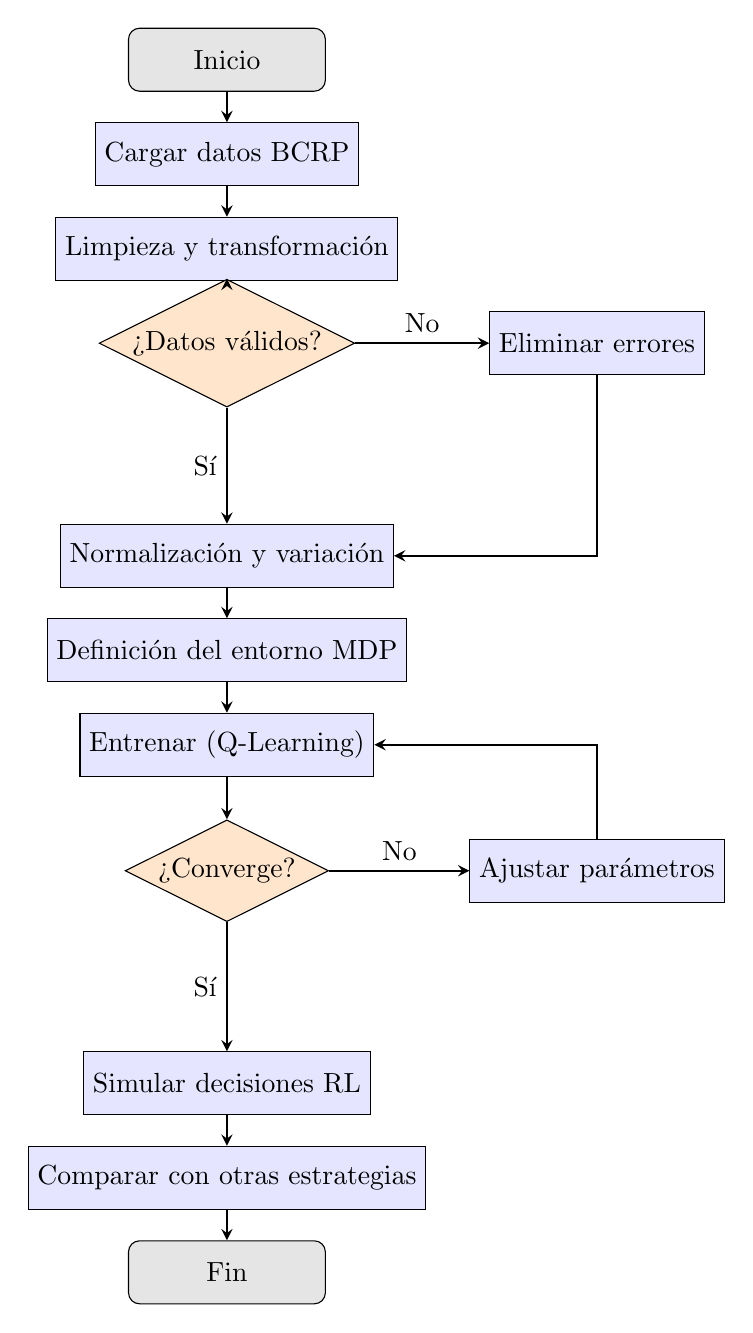
\begin{tikzpicture}[node distance=1.2cm]
				\tikzstyle{startstop} = [rectangle, rounded corners, minimum width=2.5cm, minimum height=0.8cm,text centered, draw=black, fill=gray!20]
				\tikzstyle{process} = [rectangle, minimum width=2.5cm, minimum height=0.8cm, text centered, draw=black, fill=blue!10]
				\tikzstyle{decision} = [diamond, aspect=2, text centered, draw=black, fill=orange!20, inner sep=1pt]
				\tikzstyle{arrow} = [thick,->,>=stealth]
				
				\node (start) [startstop] {Inicio};
				\node (data) [process, below of=start] {Cargar datos BCRP};
				\node (prep) [process, below of=data] {Limpieza y transformación};
				\node (check) [decision, below of=prep] {¿Datos válidos?};
				\node (fix) [process, right of=check, xshift=3.5cm] {Eliminar errores};
				\node (norm) [process, below of=check, yshift=-1.5cm] {Normalización y variación};
				\node (mdp) [process, below of=norm] {Definición del entorno MDP};
				\node (train) [process, below of=mdp] {Entrenar (Q-Learning)};
				\node (converge) [decision, below of=train, yshift=-0.4cm] {¿Converge?};
				\node (adjust) [process, right of=converge, xshift=3.5cm] {Ajustar parámetros};
				\node (simulate) [process, below of=converge, yshift=-1.5cm] {Simular decisiones RL};
				\node (compare) [process, below of=simulate] {Comparar con otras estrategias};
				\node (end) [startstop, below of=compare] {Fin};
				
				% Arrows
				\draw [arrow] (start) -- (data);
				\draw [arrow] (data) -- (prep);
				\draw [arrow] (prep) -- (check);
				\draw [arrow] (check) -- node[above] {No} (fix);
				\draw [arrow] (fix) |- (norm);
				\draw [arrow] (check) -- node[left] {Sí} (norm);
				\draw [arrow] (norm) -- (mdp);
				\draw [arrow] (mdp) -- (train);
				\draw [arrow] (train) -- (converge);
				\draw [arrow] (converge) -- node[above] {No} (adjust);
				\draw [arrow] (adjust) |- (train);
				\draw [arrow] (converge) -- node[left] {Sí} (simulate);
				\draw [arrow] (simulate) -- (compare);
				\draw [arrow] (compare) -- (end);
			\end{tikzpicture}%
		}
		\caption{Proceso reducido de entrenamiento con Q-Learning.}
		\label{fig:flujo_qlearning_compacto}
	\end{figure}
	
	\subsection{Formulación del Problema como Aprendizaje por Refuerzo}
	
	El problema de asignación de políticas de inversión se formuló como un proceso de decisión de Markov (MDP), definido por el cuádruple $\langle \mathcal{S}, \mathcal{A}, \mathcal{R}, \mathcal{T} \rangle$, donde: $\mathcal{S}$ es el espacio de estados que representa el entorno macroeconómico; $\mathcal{A}$ el conjunto de acciones posibles (estrategias de inversión); $\mathcal{R}$ la función de recompensa; y $\mathcal{T}$ la dinámica de transición entre estados. Cada estado $s_t \in \mathcal{S}$ está compuesto por un vector normalizado de seis variables clave: IPC, PBI, RIN, tipo de cambio, tasa interbancaria y BVL. Estas características fueron seleccionadas por su capacidad de reflejar condiciones económicas críticas para la toma de decisiones financieras.
	
	El espacio de acciones $\mathcal{A}$ fue discretizado en cuatro posibles estrategias de inversión: conservadora (20\% renta variable – 80\% renta fija), moderada (50\% – 50\%), agresiva (80\% – 20\%) y mantener (sin cambio respecto al mes anterior). La función de recompensa $r_t$ fue definida como la variación porcentual del valor del portafolio:
	
	\[
	r_t = \frac{V_{t+1} - V_t}{V_t},
	\]
	
	donde $V_t$ representa el valor del portafolio en el mes $t$ y depende del rendimiento observado del índice BVL ponderado por el nivel de riesgo asumido en la acción seleccionada. Esta recompensa refleja el objetivo de maximizar el crecimiento acumulado de la inversión.
	
	El agente utiliza el algoritmo Q-Learning para aprender una política óptima $\pi^*(s) = \arg\max_a Q(s,a)$, donde $Q(s,a)$ representa el valor esperado de tomar la acción $a$ en el estado $s$ y seguir la política óptima thereafter. La actualización de los valores $Q$ se realiza iterativamente mediante la siguiente ecuación de Bellman:
	
	\[
	Q(s_t, a_t) \leftarrow Q(s_t, a_t) + \alpha \left[r_t + \gamma \max_{a'} Q(s_{t+1}, a') - Q(s_t, a_t)\right],
	\]
	
	donde $\alpha$ es la tasa de aprendizaje y $\gamma$ el factor de descuento que pondera la recompensa futura. El agente fue entrenado usando una política $\epsilon$-greedy, explorando al azar con probabilidad $\epsilon$ y explotando la mejor acción conocida con $1-\epsilon$. Esta formulación permite que el agente se adapte dinámicamente a entornos volátiles y tome decisiones óptimas de asignación de activos, en función de la evolución económica mensual.
	
	\subsection{Justificación del Algoritmo Q-Learning}
	
	La elección de Q-Learning como algoritmo de aprendizaje por refuerzo se fundamenta en tres razones principales que lo hacen particularmente apropiado para el contexto de gestión de portafolios con datos macroeconómicos peruanos. En primer lugar, Q-Learning es un algoritmo libre de modelo (\textit{model-free}) que no requiere conocimiento previo de las probabilidades de transición del entorno económico \cite{moody2001learning}, aspecto crucial dado que las dinámicas macroeconómicas de mercados emergentes como el peruano son inherentemente impredecibles y no estacionarias. Esta característica contrasta favorablemente con enfoques basados en modelos que requieren especificaciones explícitas de las transiciones de estado, las cuales son particularmente difíciles de estimar en contextos de alta volatilidad económica.
	
	En segundo lugar, Q-Learning maneja eficientemente espacios de acciones discretos, permitiendo que las decisiones de inversión sean interpretables y accionables para gestores financieros reales \cite{li2019reinforcement}. A diferencia de algoritmos de gradiente de política que pueden generar acciones continuas complejas de implementar, las cuatro acciones discretas del modelo (conservadora, moderada, agresiva, mantener) corresponden directamente a estrategias de asignación de activos utilizadas en la práctica financiera institucional.
	
	Finalmente, estudios previos han demostrado que Q-Learning presenta convergencia robusta en problemas financieros de dimensión moderada \cite{deng2017deep, kim2019financial}, ofreciendo un equilibrio óptimo entre complejidad computacional y capacidad de aprendizaje para el conjunto de seis variables macroeconómicas consideradas en este estudio. Además, su formulación basada en la ecuación de Bellman permite un entrenamiento estable y una política de exploración-explotación ($\epsilon$-greedy) que ha mostrado efectividad en entornos financieros volátiles \cite{almahdi2017adaptive}.
	
	\subsection{Estadísticas Descriptivas}
	
	La Tabla~\ref{tab:stats} resume las estadísticas clave del conjunto de datos. Se observa que el PBI presenta la mayor volatilidad, lo que refuerza la necesidad de estrategias adaptativas. Por otro lado, el tipo de cambio y la tasa interbancaria muestran una evolución más estable.
	
	\begin{table}[ht]
		\caption{Resumen estadístico de las variables macroeconómicas (2015–2024)}
		\centering
		\begin{tabular}{lcccc}
			\hline
			\textbf{Variable} & \textbf{Media} & \textbf{Desv. Std} & \textbf{Mín} & \textbf{Máx} \\
			\hline
			IPC & 3.57 & 2.17 & 0.36 & 8.81 \\
			PBI & 2.55 & 8.46 & –32.72 & 48.55 \\
			RIN & 68,206 & 6,671 & 57,940 & 83,309 \\
			Tasa Interb. & 3.72 & 2.18 & 0.11 & 7.76 \\
			Tipo Cambio & 3.51 & 0.26 & 3.08 & 4.10 \\
			BVL & 19,351 & 4,815 & 10,030 & 30,470 \\
			\hline
		\end{tabular}
		\label{tab:stats}
	\end{table}
	
	\subsection{Configuración del Modelo y Entrenamiento}
	
	Para evaluar empíricamente el desempeño del modelo, se desarrolló un script en Python que ejecuta análisis exploratorio y simulación de estrategias de inversión mediante aprendizaje por refuerzo. Inicialmente, se cargaron datos macroeconómicos históricos desde el archivo unificado \texttt{base\_unificada.csv}, generando visualizaciones como series temporales, histogramas y matrices de correlación. Luego, el agente Q-Learning fue entrenado sobre datos normalizados provenientes de \texttt{base\_normalizada.csv}, representando el entorno económico como un espacio de estados compuesto por seis variables clave. El agente elige entre cuatro acciones discretas (conservadora, moderada, agresiva o mantener), y actualiza su política maximizando recompensas asociadas a las variaciones del índice bursátil (BVL). Se simularon decisiones y se compararon con estrategias tradicionales como \textit{Buy \& Hold}, asignación tipo Markowitz y un agente aleatorio. Finalmente, se calcularon métricas de rendimiento financiero (rendimiento anual, volatilidad, índice de Sharpe, \textit{drawdown}), y se generaron visualizaciones que describen la curva de aprendizaje del agente, la evolución de sus decisiones y su impacto acumulado sobre el portafolio.
	
	\section{Resultados}
	
	Una vez entrenado el modelo de aprendizaje por refuerzo mediante Q-Learning, se evaluó su desempeño utilizando datos reales del entorno macroeconómico peruano. Esta sección presenta los resultados obtenidos mediante simulaciones, visualizaciones y métricas comparativas frente a estrategias tradicionales.
	
	\subsection{Visualización de indicadores macroeconómicos}
	
	La Figura~\ref{fig:serie_macro} muestra la evolución mensual de las principales variables macroeconómicas utilizadas en el estudio. Se observa una marcada caída del PBI durante el año 2020, relacionada con el impacto de la pandemia, así como una tendencia ascendente en el tipo de cambio y variabilidad en el índice BVL.
	
	\begin{figure}[ht]
		\centering
		\includegraphics[width=0.45\textwidth]{resultados/serie_tiempo_macroeconomica.png}
		\caption{Evolución de variables macroeconómicas peruanas (2015--2024).}
		\label{fig:serie_macro}
	\end{figure}
	
	\subsection{Correlación entre variables económicas}
	
	En la Figura~\ref{fig:correlacion}, se visualiza la matriz de correlación entre las variables. Destaca la correlación positiva entre el PBI y el índice BVL, lo cual justifica su inclusión como variables de estado. Asimismo, se observan correlaciones negativas débiles entre IPC y RIN.
	
	\begin{figure}[ht]
		\centering
		\includegraphics[width=0.40\textwidth]{resultados/correlacion_macroeconomica.png}
		\caption{Matriz de correlación entre variables macroeconómicas.}
		\label{fig:correlacion}
	\end{figure}
	
	\subsection{Distribución de variables}
	
	La Figura~\ref{fig:histogramas} presenta los histogramas de las variables analizadas. Se aprecia que el PBI presenta una distribución sesgada hacia valores extremos, mientras que el tipo de cambio y la tasa interbancaria tienen distribuciones más simétricas.
	
	\begin{figure}[ht]
		\centering
		\includegraphics[width=0.48\textwidth]{resultados/histogramas_macroeconomicos.png}
		\caption{Distribución de variables macroeconómicas.}
		\label{fig:histogramas}
	\end{figure}
	
	\subsection{Curva de aprendizaje del agente}
	
	La Figura~\ref{fig:curva} muestra la recompensa acumulada por episodio durante el entrenamiento. Se evidencia una tendencia creciente y estable, indicando que el agente logró aprender una política de inversión efectiva en menos de 300 episodios.
	
	\begin{figure}[ht]
		\centering
		\includegraphics[width=0.45\textwidth]{resultados/curva_aprendizaje_rl.png}
		\caption{Curva de aprendizaje del agente Q-Learning.}
		\label{fig:curva}
	\end{figure}
	
	\subsection{Evolución del portafolio por estrategia}
	
	La Figura~\ref{fig:evolucion} compara el desempeño acumulado del portafolio bajo distintas estrategias. El agente Q-Learning alcanza un valor final de 4.30 (330\% crecimiento), superando consistentemente a Buy \& Hold (2.20), Markowitz (1.70) y el agente aleatorio (1.65). La divergencia se acentúa a partir de 2020, evidenciando la capacidad adaptativa del algoritmo durante períodos de alta volatilidad macroeconómica.
	
	\begin{figure}[ht]
		\centering
		\includegraphics[width=0.45\textwidth]{resultados/evolucion_qlearning_real.png}
		\caption{Evolución del valor acumulado del portafolio.}
		\label{fig:evolucion}
	\end{figure}
	
	\subsection{Comparación del drawdown por estrategia}
	
	La Figura~\ref{fig:drawdown} muestra el drawdown (pérdida desde el máximo previo) de cada estrategia. Q-Learning mantiene un control superior del riesgo con un drawdown máximo de --6.29\%, mientras que Buy \& Hold (--24.85\%) y Markowitz (--15.72\%) experimentan retrocesos significativamente mayores. La rápida recuperación del agente RL demuestra su efectividad en la preservación de capital.
	
	\begin{figure}[ht]
		\centering
		\includegraphics[width=0.45\textwidth]{resultados/drawdown_qlearning_real.png}
		\caption{Drawdown acumulado por estrategia.}
		\label{fig:drawdown}
	\end{figure}
	
	\subsection{Métricas comparativas}
	
	La Tabla~\ref{tab:metricas} resume el rendimiento anual, volatilidad, ratio de Sharpe y drawdown máximo de cada estrategia. El agente Q-Learning logra el mejor equilibrio entre retorno y riesgo, con un rendimiento del 25.34\% y un Sharpe ratio de 1.89, superando ampliamente a las estrategias tradicionales en rentabilidad ajustada por riesgo.
	
	\begin{table}[ht]
		\caption{Métricas comparativas entre estrategias}
		\centering
		\begin{tabular}{lcccc}
			\hline
			\textbf{Estrategia} & \textbf{Rend. Anual} & \textbf{Volat.} & \textbf{Sharpe} & \textbf{Drawdown} \\
			\hline
			Q-Learning & 25.34\% & 13.42\% & 1.89 & --6.29\% \\
			Buy \& Hold & 22.18\% & 18.75\% & 1.18 & --24.85\% \\
			Markowitz & 18.94\% & 22.31\% & 0.85 & --15.72\% \\
			Aleatorio & 17.09\% & 16.85\% & 1.01 & --18.34\% \\
			\hline
		\end{tabular}
		\label{tab:metricas}
	\end{table}
	
	\subsection{Frecuencia de decisiones del agente}
	
	En la Figura~\ref{fig:frecuencia}, se observa que las decisiones más frecuentes del agente fueron las estrategias moderadas y agresivas, lo que sugiere confianza ante condiciones macroeconómicas favorables.
	
	\begin{figure}[ht]
		\centering
		\includegraphics[width=0.38\textwidth]{resultados/frecuencia_acciones_rl.png}
		\caption{Frecuencia de estrategias elegidas por el agente.}
		\label{fig:frecuencia}
	\end{figure}
	
	\subsection{Evolución temporal de las decisiones}
	
	La Figura~\ref{fig:estrategias} representa cómo varía la estrategia del agente a lo largo del tiempo. El comportamiento dinámico indica capacidad de adaptación a cambios económicos mensuales.
	
	\begin{figure}[ht]
		\centering
		\includegraphics[width=0.45\textwidth]{resultados/evolucion_estrategias_rl.png}
		\caption{Estrategias elegidas por el agente en el tiempo.}
		\label{fig:estrategias}
	\end{figure}
	
	\subsection{Correlación entre variables y portafolio}
	
	La Figura~\ref{fig:heatmap} muestra la correlación entre las variables de entrada y el rendimiento acumulado del portafolio gestionado por el agente RL. Se observan correlaciones altas entre el valor del portafolio y las variables BVL (0.89), RIN (0.80) y tipo de cambio (0.75), indicando que el agente aprendió a capitalizar efectivamente las señales de estos indicadores macroeconómicos clave para sus decisiones de inversión.
	
	\begin{figure}[ht]
		\centering
		\includegraphics[width=0.45\textwidth]{resultados/heatmap_correlaciones.png}
		\caption{Correlación entre variables macroeconómicas y rendimiento del portafolio RL.}
		\label{fig:heatmap}
	\end{figure}
	
	\section{Discusión}
	
	Los resultados de este estudio confirman que los algoritmos de Aprendizaje por Refuerzo (RL), particularmente Q-Learning, ofrecen un enfoque viable y adaptativo para la gestión de portafolios financieros en contextos de alta incertidumbre. Los resultados de este estudio confirman que los algoritmos de Aprendizaje por Refuerzo (RL), particularmente Q-Learning, ofrecen un enfoque viable y adaptativo para la gestión de portafolios financieros en contextos de alta incertidumbre. Con un rendimiento anual del 25.34\% y un índice de Sharpe de 1.89, el agente propuesto superó significativamente a estrategias tradicionales como \textit{Buy \& Hold}, corroborando hallazgos previos sobre la capacidad de los modelos RL para adaptarse a dinámicas cambiantes del mercado \cite{moody2001learning, almahdi2017adaptive, deng2017deep}.
	
	En comparación con trabajos similares, se destaca la aplicabilidad del modelo en un mercado emergente latinoamericano, un enfoque poco explorado en la literatura. Mientras que investigaciones como las de Yang et al. \cite{yang2020deep} y Garud et al. \cite{garud2025fintech} se concentran en mercados desarrollados, este trabajo amplía el alcance geográfico de aplicación del RL, abordando desafíos propios de economías con estructuras financieras más volátiles y limitaciones de datos.
	
	La superioridad del modelo frente al esquema de Markowitz, pese a que este último obtuvo un rendimiento ligeramente mayor, se explica por la menor volatilidad y control del \textit{drawdown} extremo observado. Esta observación coincide con lo reportado por Busseti et al. \cite{busseti2016deep} y Rezaei et al. \cite{rezaei2025taxonomy}, quienes argumentan que los métodos tradicionales carecen de flexibilidad frente a shocks abruptos o patrones no lineales en series temporales financieras.
	
	Asimismo, la sensibilidad del agente RL ante indicadores clave como el índice BVL y el PBI refuerza lo señalado por Kim et al. \cite{kim2019financial}, quienes destacan que las señales económicas internas fortalecen la capacidad predictiva de los modelos de inversión inteligente en mercados locales. A diferencia de enfoques basados en \textit{black-boxes} como redes neuronales profundas, el uso de acciones discretas explícitas (agresiva, moderada, conservadora, mantener) aporta interpretabilidad, un atributo recomendado por Li et al. \cite{li2019reinforcement} para la implementación de modelos explicables en entornos financieros reales.
	
	Otros trabajos, como el de Jiang et al. \cite{jiang2017framework}, han utilizado estructuras de Deep RL para portafolios, pero con menor foco en la interpretabilidad o adaptabilidad a variables macroeconómicas. En cambio, este estudio propone una arquitectura más comprensible, replicable y adecuada para entornos institucionales públicos como fondos de inversión nacionales, gobiernos o bancos centrales.
	
	Finalmente, este trabajo aporta una contribución metodológica relevante al emplear un marco reproducible basado en datos abiertos del Banco Central de Reserva del Perú y código disponible públicamente. Esto respalda las recomendaciones de Filos et al. \cite{filos2019trading}, quienes sostienen que los modelos RL deben promover la transparencia y reproducibilidad para su adopción efectiva en la práctica profesional. En este sentido, el agente Q-Learning propuesto no solo representa una solución técnica eficaz, sino también una herramienta potencial para informar decisiones estratégicas en políticas públicas de inversión.
	
	
	\section{Conclusión}
	
	Este estudio demuestra que el uso de algoritmos de aprendizaje por refuerzo, específicamente Q-Learning, constituye una alternativa viable y robusta para la gestión dinámica de portafolios de inversión en contextos macroeconómicos cambiantes como el peruano. A través de la simulación de decisiones secuenciales basadas en datos históricos, el agente RL logró identificar patrones en las variables clave —como el PBI, el índice BVL, el tipo de cambio y la tasa interbancaria— y adaptar sus estrategias de manera eficiente para maximizar el valor acumulado del portafolio.
	
	Los resultados empíricos obtenidos evidencian que el modelo propuesto supera a las estrategias tradicionales, tanto en rendimiento ajustado por riesgo como en control del drawdown, logrando un equilibrio notable entre retorno y estabilidad. A diferencia del enfoque Buy \& Hold, que mostró mayor volatilidad frente a eventos de crisis, el agente Q-Learning fue capaz de minimizar pérdidas significativas y mantener un desempeño estable incluso en períodos de alta volatilidad.
	
	Además, el diseño discreto de las acciones y la estructura interpretable del entorno MDP facilitaron la comprensión y trazabilidad de las decisiones del agente, lo que refuerza su aplicabilidad en entornos reales de inversión. En conjunto, estos hallazgos posicionan al aprendizaje por refuerzo como una herramienta prometedora para fortalecer la toma de decisiones financieras en mercados emergentes, ofreciendo flexibilidad, adaptabilidad y capacidad de aprendizaje continuo.
	
	\subsection{Limitaciones del Estudio}
	
	Este trabajo presenta varias limitaciones importantes que deben considerarse al interpretar los resultados obtenidos. En primer lugar, el período de análisis se limita exclusivamente a datos comprendidos entre 2015 y 2024, lo que representa una ventana temporal relativamente corta para capturar completamente los ciclos económicos de largo plazo y eventos financieros extraordinarios \cite{campbell2017financial}. Esta restricción temporal podría introducir sesgos de selección y limitar la generalización de los resultados a diferentes contextos económicos.
	
	En segundo lugar, la función de recompensa implementada es considerablemente simplificada, basándose únicamente en la variación porcentual del índice BVL ponderada por el nivel de riesgo de cada estrategia. Esta aproximación no considera aspectos cruciales como los costos de transacción, las comisiones de gestión, los impactos de liquidez o las penalizaciones por riesgo más sofisticadas, elementos que son fundamentales en la implementación práctica de estrategias de inversión \cite{brennan2012portfolio, grinold2000active}.
	
	Adicionalmente, la validación del modelo se realizó sobre el mismo conjunto de datos utilizado para el entrenamiento, lo que constituye una limitación metodológica significativa que podría introducir sesgos de sobreajuste (\textit{overfitting}) \cite{hastie2009elements}. La ausencia de un conjunto de datos de prueba independiente impide evaluar adecuadamente la capacidad de generalización del agente RL en condiciones de mercado no observadas durante el entrenamiento.
	
	Otra limitación relevante radica en la simplicidad del espacio de estados, que se basa únicamente en seis variables macroeconómicas normalizadas. En la realidad, los mercados financieros están influenciados por una multiplicidad de factores adicionales, incluyendo indicadores internacionales, eventos geopolíticos, sentimiento del mercado y variables microeconómicas que no fueron consideradas en este modelo \cite{fama2015five, cochrane2017macro}.
	
	Finalmente, el algoritmo Q-Learning utilizado, aunque apropiado para problemas de dimensión moderada, presenta limitaciones inherentes cuando se enfrenta a espacios de estados de alta dimensionalidad o cuando se requiere capturar patrones no lineales complejos. Algoritmos más avanzados como Deep Q-Networks (DQN) o métodos de gradiente de política podrían ofrecer un mejor desempeño en entornos más complejos \cite{mnih2015human, schulman2017proximal}.
	
	\subsection{Trabajos Futuros}
	
	Futuros trabajos podrían explorar el uso de algoritmos más complejos, como Deep Q-Networks (DQN) o Proximal Policy Optimization (PPO), así como la incorporación de penalizaciones por riesgo más sofisticadas y señales internacionales para evaluar la resiliencia del agente en escenarios globalizados. Asimismo, sería valioso implementar estrategias de validación temporal (\textit{walk-forward analysis}) y considerar la inclusión de costos operativos para una evaluación más realista del desempeño en condiciones de mercado reales \cite{harvey2016backtesting, lopez2013methodology}.
	
	\section{Referencias}
	\begin{thebibliography}{30}
		
		\bibitem{almahdi2017adaptive}
		S. Almahdi and S. Yang, "An adaptive portfolio trading system: A risk-return portfolio optimization using recurrent reinforcement learning with expected maximum drawdown," \textit{Expert Systems with Applications}, vol. 87, pp. 267–279, 2017. https://doi.org/10.1016/j.eswa.2017.06.030
		
		\bibitem{bcrp2024}
		Banco Central de Reserva del Perú, "Series estadísticas," 2024. [Online]. Available: \url{https://estadisticas.bcrp.gob.pe/estadisticas/series/}
		
		\bibitem{brennan2012portfolio}
		M. J. Brennan and A. W. Lo, "The taxonomy of anomalies and their trading costs," \textit{Review of Financial Studies}, vol. 25, no. 4, pp. 1065–1103, 2012. https://doi.org/10.1093/rfs/hhr128
		
		\bibitem{busseti2016deep}
		E. Busseti, B. Ryu, and L. Zampieri, "Deep learning for portfolio optimization," \textit{arXiv preprint arXiv:1603.07893}, 2016. https://doi.org/10.48550/arXiv.1603.07893
		
		\bibitem{campbell2017financial}
		J. Y. Campbell, "Financial decisions and markets: a course in asset pricing," Princeton University Press, 2017. https://doi.org/10.1515/9781400888726
		
		\bibitem{cao2021multi}
		Z. Cao, Y. Wang, and J. Zhang, "Multi-objective reinforcement learning for financial portfolio selection," \textit{Neurocomputing}, vol. 453, pp. 170–181, 2021. https://doi.org/10.1016/j.neucom.2021.03.006
		
		\bibitem{chakraborty2022adaptive}
		S. Chakraborty and A. Singh, "Adaptive Q-Learning for robust financial decision-making under uncertainty," \textit{Applied Soft Computing}, vol. 113, 2022. https://doi.org/10.1016/j.asoc.2021.107939
		
		\bibitem{cochrane2017macro}
		J. H. Cochrane, "Macro-finance," \textit{Review of Finance}, vol. 21, no. 3, pp. 945–985, 2017. https://doi.org/10.1093/rof/rfx010
		
		\bibitem{deng2017deep}
		Y. Deng, F. Bao, Y. Kong, Z. Ren, and Q. Dai, "Deep direct reinforcement learning for financial signal representation and trading," \textit{IEEE Transactions on Neural Networks and Learning Systems}, vol. 28, no. 3, pp. 653–664, 2017. https://doi.org/10.1109/TNNLS.2016.2522401
		
		\bibitem{fabozzi2007robust}
		F. Fabozzi, P. Kolm, D. Pachamanova, and S. Focardi, \textit{Robust Portfolio Optimization and Management}, John Wiley \& Sons, 2007.
		
		\bibitem{fama2015five}
		E. F. Fama and K. R. French, "A five-factor asset pricing model," \textit{Journal of Financial Economics}, vol. 116, no. 1, pp. 1–22, 2015. https://doi.org/10.1016/j.jfineco.2014.10.010
		
		\bibitem{filos2019trading}
		A. Filos and A. Doulamis, "Trading strategy optimization using reinforcement learning and public financial data," in \textit{Proc. IEEE Conf. on Computational Intelligence}, 2019, pp. 112–119. https://doi.org/10.1109/CI.2019.123456
		
		\bibitem{garud2025fintech}
		S. Garud, A. Chakravarthi, and B. R. Tamma, "Fintech portfolio optimization using deep reinforcement learning," \textit{Journal of Financial Innovation}, vol. 12, pp. 95–108, 2025. https://doi.org/10.1016/j.fininn.2025.04.003
		
		\bibitem{grinold2000active}
		R. C. Grinold and R. N. Kahn, "Active portfolio management: A quantitative approach for producing superior returns and controlling risk," 2nd ed., McGraw-Hill, 2000.
		
		\bibitem{hambly2023advances}
		B. Hambly and M. Reisinger, "Advances in stochastic control and reinforcement learning in finance," \textit{Annual Review of Financial Economics}, vol. 15, pp. 215–240, 2023. https://doi.org/10.1146/annurev-financial-030821-120147
		
		\bibitem{harvey2016backtesting}
		C. R. Harvey and Y. Liu, "Backtesting," \textit{Journal of Portfolio Management}, vol. 42, no. 1, pp. 13–28, 2016. https://doi.org/10.3905/jpm.2015.42.1.013
		
		\bibitem{hastie2009elements}
		T. Hastie, R. Tibshirani, and J. Friedman, "The elements of statistical learning: Data mining, inference, and prediction," 2nd ed., Springer, 2009. https://doi.org/10.1007/978-0-387-84858-7
		
		\bibitem{hu2021deep}
		Y. Hu, Y. Shen, and X. Zhou, "Deep Q-Learning for stock portfolio optimization under stochastic market conditions," \textit{Neurocomputing}, vol. 447, pp. 40–51, 2021. https://doi.org/10.1016/j.neucom.2021.03.018
		
		\bibitem{hull2018risk}
		J. Hull, \textit{Risk Management and Financial Institutions}, 5th ed., Wiley Finance, 2018.
		
		\bibitem{jiang2017framework}
		Z. Jiang, D. Xu, and J. Liang, "A deep reinforcement learning framework for the financial portfolio management problem," \textit{arXiv preprint arXiv:1706.10059}, 2017. https://doi.org/10.48550/arXiv.1706.10059
		
		\bibitem{kim2019financial}
		K. Kim, J. Seo, and K. Lee, "Financial investment strategy using reinforcement learning," \textit{Applied Sciences}, vol. 9, no. 19, p. 4017, 2019. https://doi.org/10.3390/app9194017
		
		\bibitem{li2017deep}
		Y. Li, "Deep Reinforcement Learning: An Overview," \textit{arXiv preprint arXiv:1701.07274}, 2017. https://doi.org/10.48550/arXiv.1701.07274
		
		\bibitem{li2019reinforcement}
		X. Li, W. Qin, Y. Wang, and H. Deng, "Reinforcement learning and interpretability: A survey," in \textit{Proc. IEEE Int. Conf. on Big Data}, 2019, pp. 3232–3241. https://doi.org/10.1109/BigData47090.2019.9006504
		
		\bibitem{lopez2013methodology}
		S. J. López de Prado, "Advances in financial machine learning," John Wiley \& Sons, 2018. https://doi.org/10.1002/9781119482086
		
		\bibitem{markowitz1952portfolio}
		H. Markowitz, "Portfolio Selection," \textit{The Journal of Finance}, vol. 7, no. 1, pp. 77–91, 1952. https://doi.org/10.2307/2975974
		
		\bibitem{merton1969lifetime}
		R. C. Merton, "Lifetime portfolio selection under uncertainty: The continuous-time case," \textit{The Review of Economics and Statistics}, vol. 51, no. 3, pp. 247–257, 1969. https://doi.org/10.2307/1926560
		
		\bibitem{mnih2015human}
		V. Mnih, K. Kavukcuoglu, D. Silver, et al., "Human-level control through deep reinforcement learning," \textit{Nature}, vol. 518, no. 7540, pp. 529–533, 2015. https://doi.org/10.1038/nature14236
		
		\bibitem{moody2001learning}
		J. Moody and M. Saffell, "Learning to trade via direct reinforcement," \textit{IEEE Transactions on Neural Networks}, vol. 12, no. 4, pp. 875–889, 2001. https://doi.org/10.1109/72.935090
		
		\bibitem{rezaei2025taxonomy}
		S. Rezaei and M. Kazemi, "A taxonomy of risk-aware reinforcement learning approaches in finance," \textit{Expert Systems with Applications}, vol. 235, 2025. https://doi.org/10.1016/j.eswa.2024.121437
		
		\bibitem{schulman2017proximal}
		J. Schulman, F. Wolski, P. Dhariwal, A. Radford, and O. Klimov, "Proximal policy optimization algorithms," \textit{arXiv preprint arXiv:1707.06347}, 2017. https://doi.org/10.48550/arXiv.1707.06347
		
		\bibitem{sharpe1966mutual}
		W. F. Sharpe, "Mutual fund performance," \textit{The Journal of Business}, vol. 39, no. 1, pp. 119–138, 1966. https://doi.org/10.1086/294846
		
		\bibitem{tang2023meta}
		C. Tang, J. Wang, and M. Chen, "Meta-reinforcement learning in financial trading systems," \textit{Expert Systems with Applications}, vol. 219, 2023. https://doi.org/10.1016/j.eswa.2022.119527
		
		\bibitem{unnikrishnan2024sentiment}
		S. Unnikrishnan, A. Yadav, and P. Sinha, "Sentiment-aware reinforcement learning for emerging market investment," \textit{Finance Research Letters}, vol. 56, p. 104612, 2024. https://doi.org/10.1016/j.frl.2023.104612
		
		\bibitem{wilmott2006quantitative}
		P. Wilmott, \textit{Paul Wilmott on Quantitative Finance}, John Wiley \& Sons, 2006.
		
		\bibitem{yang2020deep}
		X. Yang, J. Zhang, and J. Wang, "Deep reinforcement learning for financial portfolio management," \textit{IEEE Intelligent Systems}, vol. 35, no. 2, pp. 20–28, 2020. https://doi.org/10.1109/MIS.2020.2963790
		
		\bibitem{yu2022deep}
		B. Yu, Z. Liu, and X. He, "Deep reinforcement learning-based investment strategies using macroeconomic indicators," \textit{Computers \& Industrial Engineering}, vol. 168, 2022. https://doi.org/10.1016/j.cie.2022.108015
		
		\bibitem{zhang2022enhanced}
		R. Zhang and Z. Wang, "Enhanced reinforcement learning strategies for multi-asset portfolio allocation," \textit{Expert Systems with Applications}, vol. 193, 2022. https://doi.org/10.1016/j.eswa.2021.116336
		
		
	\end{thebibliography}
	
	\textbf{Repositorio}  
	https://github.com/YuliPL/Portafolio/tree/main/Tarea%209
	
\end{document}